This chapter uses data from a cross-over study by Dai, Lov,
Martin-Arrowsmith et al.~\cite{dai2022insect}. The trial measured
various outcomes after ingesting a protein-based beverage, comparing
between beef- or insect-derived proteins. 20 subjects were randomised
into either the cricket-beef (C-B) sequence or the beef-cricket (B-C)
sequence. For the following examples, we focus on data collected on
insulin levels 300 minutes after ingestion.

We will apply the methods described in the preceding chapters to the
data, in order to determine whether there is a difference between the
beef- or insect-derived proteins (in terms of resulting insulin levels).

\section{Standard Cross-over Design}\label{standard-cross-over-design}

\subsection{Data Structure}\label{data-structure}

Most data manipulation and visualisation is performed using the
\texttt{tidyverse} package (which includes \texttt{ggplot}); other
packages used are indicated where applicable. It is important that the
columns for subject, sequence, period and treatment are treated as
factors (instead of continuous).

The data were collected in `long' format, where we have a column for
period and a column for the measurement (see table
\ref{tab:data-long-demo}). For some plots it is easier for the data to
be in `wide' format (see table \ref{tab:data-wide-demo}); this can
easily be achieved with \texttt{tidyr::pivot\_wider()}.

\begin{table}
\centering
\caption{\label{tab:data-long-demo}Subsample of Data in 'Long' Format}
\centering
\begin{tabular}[t]{llllr}
\toprule
Subject & Sequence & Period & Treatment & Insulin\\
\midrule
1 & C-B & 1 & CRICKET & 18.3\\
1 & C-B & 2 & BEEF & 14.1\\
2 & C-B & 1 & CRICKET & 14.7\\
2 & C-B & 2 & BEEF & 24.7\\
4 & C-B & 1 & CRICKET & 45.9\\
\bottomrule
\end{tabular}
\end{table}

\begin{Shaded}
\begin{Highlighting}[]
\NormalTok{data.wide }\OtherTok{\textless{}{-}}\NormalTok{ data }\SpecialCharTok{\%\textgreater{}\%}
  \FunctionTok{pivot\_wider}\NormalTok{(}\AttributeTok{id\_cols =} \FunctionTok{c}\NormalTok{(Subject, Sequence),}
              \AttributeTok{names\_from =}\NormalTok{ Period, }\AttributeTok{values\_from =}\NormalTok{ Insulin,}
              \AttributeTok{names\_prefix =} \StringTok{"Period"}\NormalTok{)}
\end{Highlighting}
\end{Shaded}

\begin{table}
\centering
\caption{\label{tab:data-wide-demo}Subsample of Data in 'Wide' Format}
\centering
\begin{tabular}[t]{llrr}
\toprule
Subject & Sequence & Period1 & Period2\\
\midrule
1 & C-B & 18.3 & 14.1\\
2 & C-B & 14.7 & 24.7\\
4 & C-B & 45.9 & 35.8\\
5 & C-B & 46.1 & 38.6\\
7 & C-B & 17.6 & 17.7\\
\bottomrule
\end{tabular}
\end{table}

\subsection{Summarising the Data}\label{summarising-the-data}

Now we can move on to the summary tables and plots, to gain a better
understanding of the data. First, the summary table; initial summaries
by sequence and period can be easily calculated using
\texttt{dplyr::summarise()}, but the aggregated total summaries (total,
by period and by sequence) must be calculated separately and joined to
compile the full summary table.

\begin{Shaded}
\begin{Highlighting}[]
\CommentTok{\# Summary by period \& sequence}
\NormalTok{summary.period.sequence }\OtherTok{\textless{}{-}}\NormalTok{ data.wide }\SpecialCharTok{\%\textgreater{}\%}
  \FunctionTok{group\_by}\NormalTok{(Sequence) }\SpecialCharTok{\%\textgreater{}\%}
  \FunctionTok{summarise}\NormalTok{(}\AttributeTok{Subjects =} \FunctionTok{n}\NormalTok{(),}
            \AttributeTok{meanPeriod1 =} \FunctionTok{mean}\NormalTok{(Period1),}
            \AttributeTok{sdPeriod1 =} \FunctionTok{sd}\NormalTok{(Period1),}
            \AttributeTok{meanPeriod2 =} \FunctionTok{mean}\NormalTok{(Period2),}
            \AttributeTok{sdPeriod2 =} \FunctionTok{sd}\NormalTok{(Period2))}

\CommentTok{\# Summary by sequence}
\NormalTok{summary.sequence }\OtherTok{\textless{}{-}}\NormalTok{ data }\SpecialCharTok{\%\textgreater{}\%}
  \FunctionTok{group\_by}\NormalTok{(Sequence) }\SpecialCharTok{\%\textgreater{}\%}
  \FunctionTok{summarise}\NormalTok{(}\AttributeTok{meanOverall =} \FunctionTok{mean}\NormalTok{(Insulin),}
            \AttributeTok{sdOverall =} \FunctionTok{sd}\NormalTok{(Insulin))}

\CommentTok{\# Summary by period}
\NormalTok{summary.period }\OtherTok{\textless{}{-}}\NormalTok{ data }\SpecialCharTok{\%\textgreater{}\%}
  \FunctionTok{group\_by}\NormalTok{(Period) }\SpecialCharTok{\%\textgreater{}\%}
  \FunctionTok{summarise}\NormalTok{(}\AttributeTok{meanPeriod =} \FunctionTok{mean}\NormalTok{(Insulin),}
            \AttributeTok{sdPeriod =} \FunctionTok{sd}\NormalTok{(Insulin)) }\SpecialCharTok{\%\textgreater{}\%}
  \FunctionTok{pivot\_wider}\NormalTok{(}\AttributeTok{names\_from =}\NormalTok{ Period, }\AttributeTok{values\_from =} \FunctionTok{c}\NormalTok{(meanPeriod, sdPeriod),}
              \AttributeTok{names\_sep =} \StringTok{""}\NormalTok{) }\SpecialCharTok{\%\textgreater{}\%}
  \FunctionTok{mutate}\NormalTok{(}\AttributeTok{Sequence =} \StringTok{"Total"}\NormalTok{, }\AttributeTok{Subjects =} \FunctionTok{n\_distinct}\NormalTok{(data}\SpecialCharTok{$}\NormalTok{Subject),}
         \AttributeTok{meanOverall =} \FunctionTok{mean}\NormalTok{(data}\SpecialCharTok{$}\NormalTok{Insulin),}
         \AttributeTok{sdOverall =} \FunctionTok{sd}\NormalTok{(data}\SpecialCharTok{$}\NormalTok{Insulin),}
         \AttributeTok{.before =}\NormalTok{ meanPeriod1)}

\CommentTok{\# Combine tables together}
\NormalTok{table1 }\OtherTok{\textless{}{-}} \FunctionTok{inner\_join}\NormalTok{(summary.sequence, summary.period.sequence,}
                     \AttributeTok{by =} \StringTok{"Sequence"}\NormalTok{) }\SpecialCharTok{\%\textgreater{}\%}
  \FunctionTok{bind\_rows}\NormalTok{(summary.period) }\SpecialCharTok{\%\textgreater{}\%}
  \FunctionTok{relocate}\NormalTok{(Subjects, }\AttributeTok{.after =}\NormalTok{ Sequence)}
\end{Highlighting}
\end{Shaded}

\begin{table}
\centering
\caption{\label{tab:table1}Summary Table}
\centering
\resizebox{\ifdim\width>\linewidth\linewidth\else\width\fi}{!}{
\begin{tabular}[t]{l>{}r|r>{}r|rrrr}
\toprule
\multicolumn{2}{c}{ } & \multicolumn{2}{c}{Overall} & \multicolumn{2}{c}{Period 1} & \multicolumn{2}{c}{Period 2} \\
\cmidrule(l{3pt}r{3pt}){3-4} \cmidrule(l{3pt}r{3pt}){5-6} \cmidrule(l{3pt}r{3pt}){7-8}
Sequence & Subjects & Mean & SD & Mean & SD & Mean & SD\\
\midrule
C-B & 10 & 24.55 & 14.43 & 25.13 & 16.07 & 23.97 & 13.45\\
B-C & 10 & 23.12 & 11.11 & 25.84 & 13.83 & 20.40 & 7.27\\
\midrule\\
Total & 20 & 23.84 & 12.74 & 25.48 & 14.60 & 22.18 & 10.68\\
\bottomrule
\end{tabular}}
\end{table}

\subsubsection{Visualisations}\label{visualisations}

We start with a boxplot (see figure \ref{fig:summary-boxplot}) and
groups-by-periods plot (see figure \ref{fig:groups-by-periods}),
summarising the results by sequence and period. The subject-profile plot
(see figure \ref{fig:subject-profile}) provides a subject-level
visualisation.
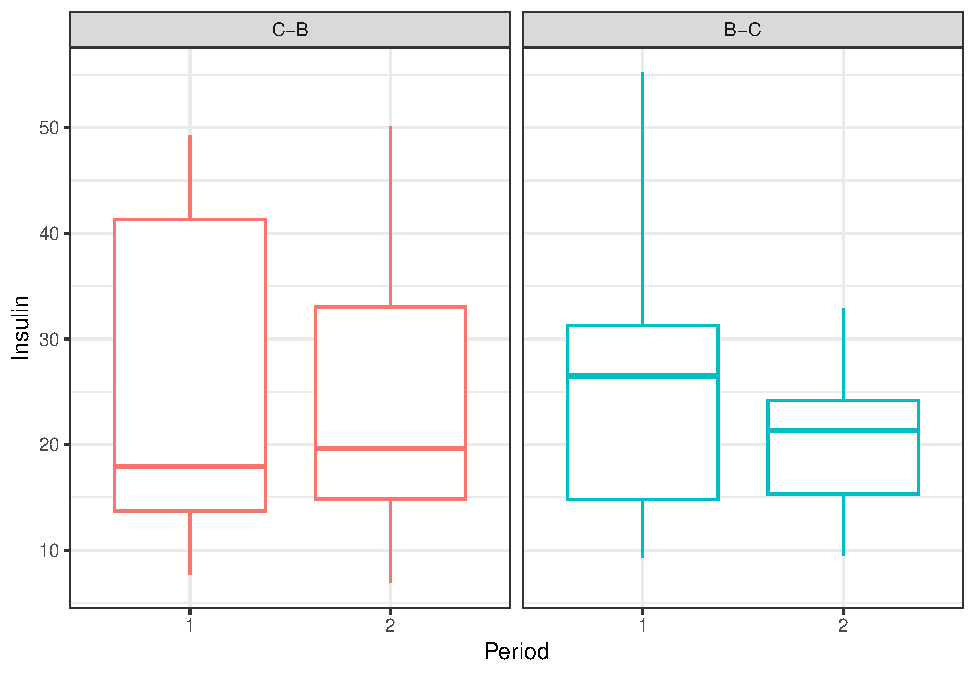
\includegraphics{ch4_files/figure-latex/summary-boxplot-1.pdf}

\begin{figure}
\centering
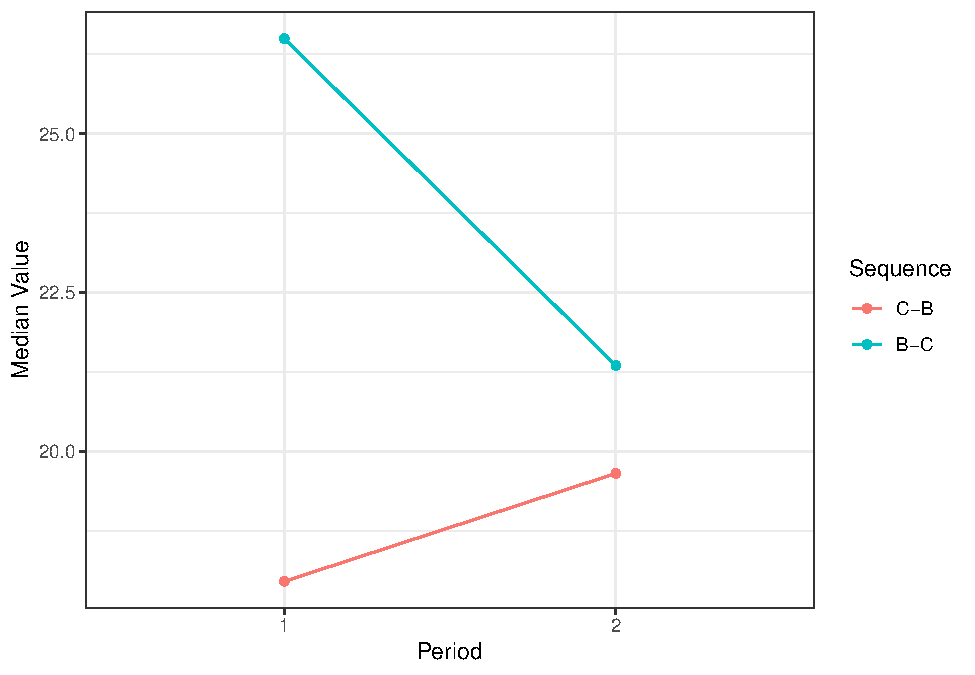
\includegraphics{ch4_files/figure-latex/groups-by-periods-1.pdf}
\caption{Groups-by-Periods Plot}
\end{figure}

\begin{figure}
\centering
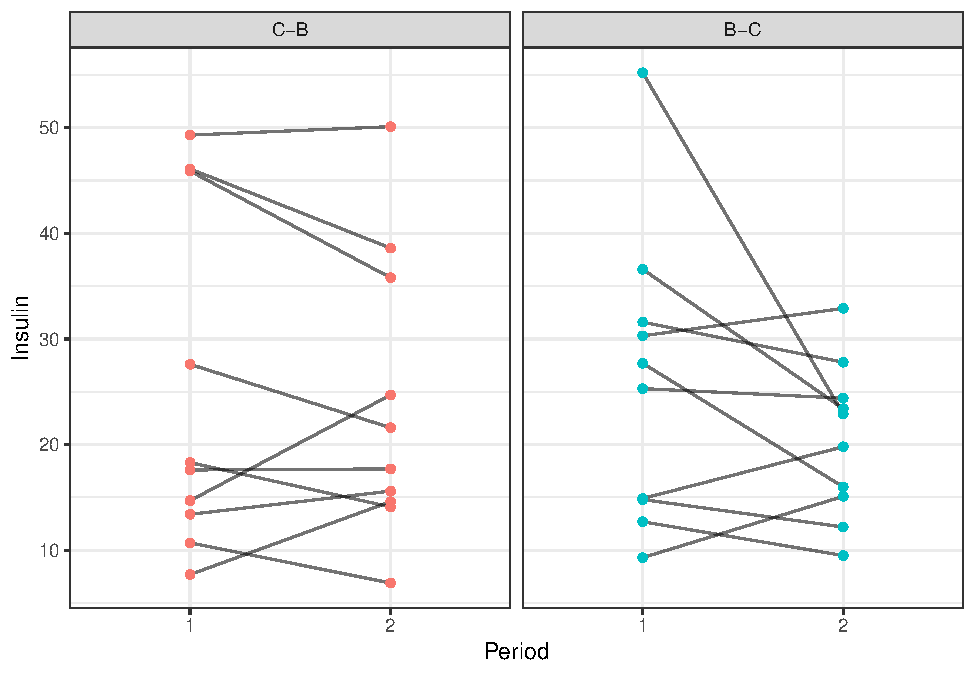
\includegraphics{ch4_files/figure-latex/subject-profile-1.pdf}
\caption{Subject-Profile Plot}
\end{figure}

Now we examine potential treatment differences with figures
\ref{fig:period-by-period} and \ref{fig:centroids}. Due to the
relatively small sample size, it is difficult to extract any potential
trends from the data at this stage. Notice, however, that there are a
number of potential outliers in each sequence, which appear to be
influencing the centroids (which are calculated using means).

\begin{figure}
\centering
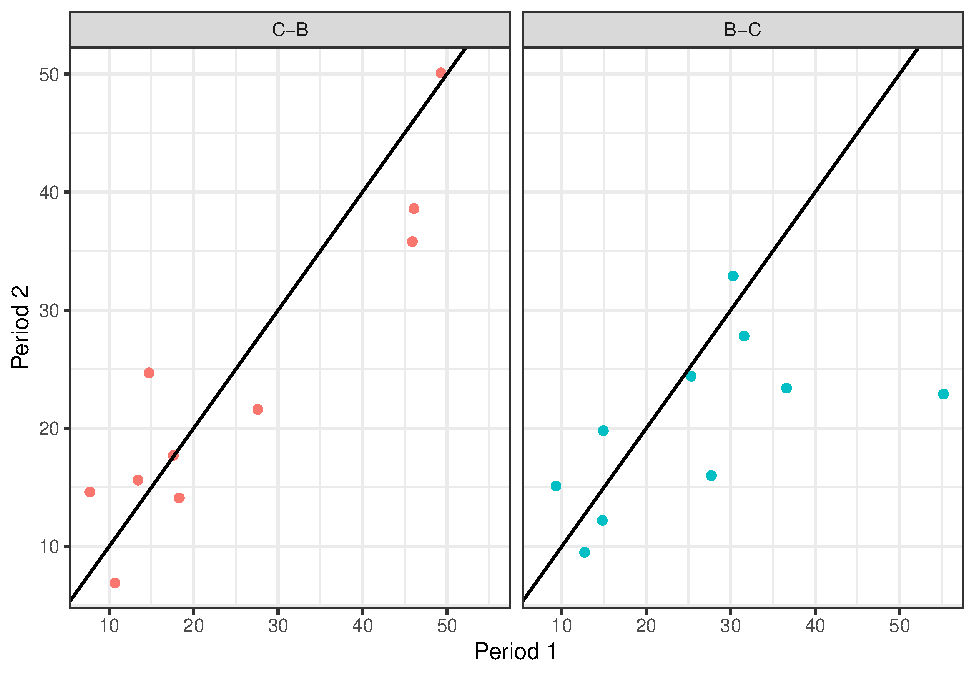
\includegraphics{ch4_files/figure-latex/period-by-period-1.pdf}
\caption{Period-by-Period Plot}
\end{figure}

\begin{figure}
\centering
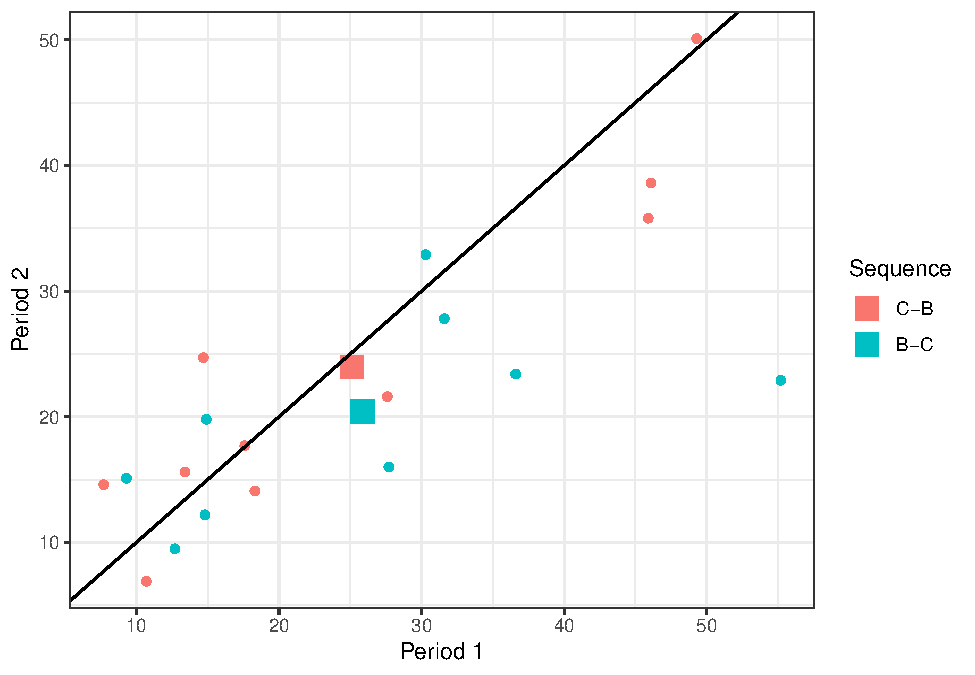
\includegraphics{ch4_files/figure-latex/centroids-1.pdf}
\caption{Period-by-Period Plot with Centroids}
\end{figure}

Reconstructing the plot, using median centroids instead (see figure
\ref{fig:centroids-median}), confirms this suspicion and provides more
insight. We see that the median centroids appear on opposite sides of
the line, with some vertical separation, indicating a potential
difference between the treatments.

\begin{figure}
\centering
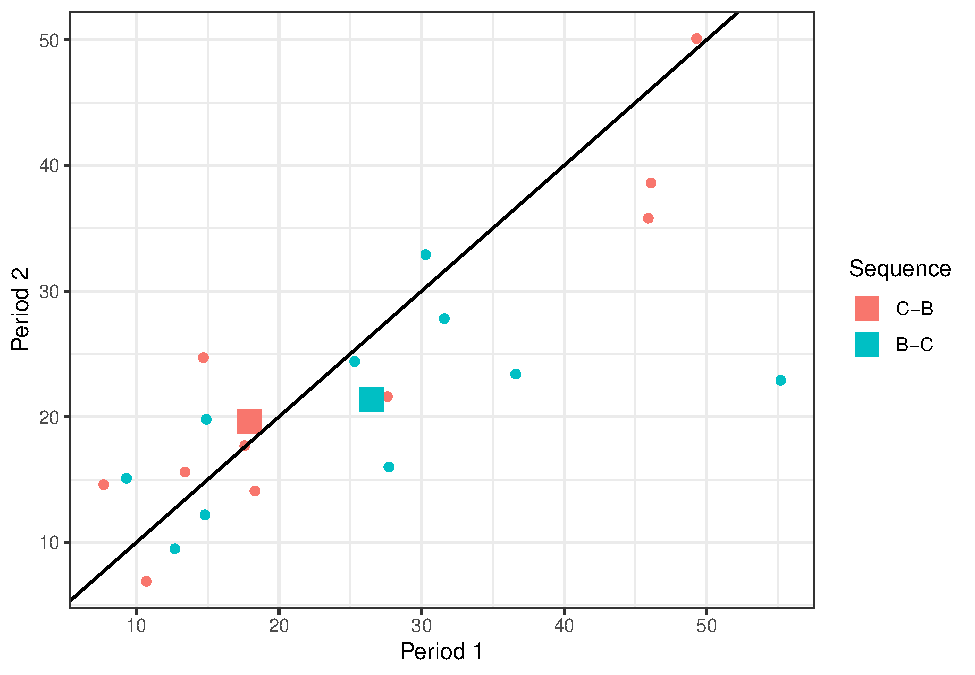
\includegraphics{ch4_files/figure-latex/centroids-median-1.pdf}
\caption{Period-by-Period Plot with Median Centroids}
\end{figure}

\subsection{Modelling for Treatment
Differences}\label{modelling-for-treatment-differences}

First we construct an ANOVA table, to verify that the other effects do
not overly influence the data. This can be easily done using the
built-in \texttt{aov()} function on the data in `long' format,
specifying the linear model equation as an argument. The ANOVA table
itself can be obtained using the \texttt{summary()} function on the
\texttt{aov} object. The resulting table is shown in table
\ref{tab:anova-table}.

\begin{Shaded}
\begin{Highlighting}[]
\NormalTok{anova.table }\OtherTok{\textless{}{-}} \FunctionTok{aov}\NormalTok{(Insulin }\SpecialCharTok{\textasciitilde{}}\NormalTok{ Treatment }\SpecialCharTok{+}\NormalTok{ Period }\SpecialCharTok{+}\NormalTok{ Sequence }\SpecialCharTok{+}\NormalTok{ Subject, }\AttributeTok{data =}\NormalTok{ data) }\SpecialCharTok{\%\textgreater{}\%}
  \FunctionTok{summary}\NormalTok{()}
\end{Highlighting}
\end{Shaded}

\begin{table}[ht]
\centering
\begin{tabular}{lrrrrr}
  \toprule
 & Df & Sum Sq & Mean Sq & F value & Pr($>$F) \\ 
  \midrule
Treatment   & 1 & 45.80 & 45.80 & 1.08 & 0.3116 \\ 
  Period      & 1 & 108.90 & 108.90 & 2.58 & 0.1258 \\ 
  Sequence    & 1 & 20.45 & 20.45 & 0.48 & 0.4955 \\ 
  Subject     & 18 & 5390.02 & 299.45 & 7.09 & 0.0001 \\ 
  Residuals   & 18 & 760.56 & 42.25 &  &  \\ 
   \bottomrule
\end{tabular}
\caption{ANOVA on Linear Model} 
\end{table}

We see that none of the other effects are significant, so we can safely
move on to test for treatment differences. The mixed model can be
implemented using the \texttt{lme4::lmer()} function, in conjunction
with the \texttt{lmerTest} package (for p-values). We specify the linear
model as normal, with the \texttt{(1\textbar{}Subject)} term specifying
that Subject is a random effect.

\begin{Shaded}
\begin{Highlighting}[]
\FunctionTok{library}\NormalTok{(lme4)}
\FunctionTok{library}\NormalTok{(lmerTest)}
\NormalTok{mixed.model }\OtherTok{\textless{}{-}} \FunctionTok{lmer}\NormalTok{(Insulin }\SpecialCharTok{\textasciitilde{}}\NormalTok{ Treatment }\SpecialCharTok{+}\NormalTok{ Period }\SpecialCharTok{+}\NormalTok{ Sequence }\SpecialCharTok{+}\NormalTok{ (}\DecValTok{1} \SpecialCharTok{|}\NormalTok{ Subject),}
                    \AttributeTok{data =}\NormalTok{ data)}
\end{Highlighting}
\end{Shaded}

\begin{longtable}[]{@{}
  >{\raggedright\arraybackslash}p{(\columnwidth - 10\tabcolsep) * \real{0.2090}}
  >{\raggedleft\arraybackslash}p{(\columnwidth - 10\tabcolsep) * \real{0.1343}}
  >{\raggedleft\arraybackslash}p{(\columnwidth - 10\tabcolsep) * \real{0.1642}}
  >{\raggedleft\arraybackslash}p{(\columnwidth - 10\tabcolsep) * \real{0.0896}}
  >{\raggedleft\arraybackslash}p{(\columnwidth - 10\tabcolsep) * \real{0.1194}}
  >{\raggedleft\arraybackslash}p{(\columnwidth - 10\tabcolsep) * \real{0.2836}}@{}}
\caption{Estimates for Mixed Model}\tabularnewline
\toprule\noalign{}
\begin{minipage}[b]{\linewidth}\raggedright
\end{minipage} & \begin{minipage}[b]{\linewidth}\raggedleft
Estimate
\end{minipage} & \begin{minipage}[b]{\linewidth}\raggedleft
Std. Error
\end{minipage} & \begin{minipage}[b]{\linewidth}\raggedleft
df
\end{minipage} & \begin{minipage}[b]{\linewidth}\raggedleft
t value
\end{minipage} & \begin{minipage}[b]{\linewidth}\raggedleft
Pr(\textgreater\textbar t\textbar)
\end{minipage} \\
\midrule\noalign{}
\endfirsthead
\toprule\noalign{}
\begin{minipage}[b]{\linewidth}\raggedright
\end{minipage} & \begin{minipage}[b]{\linewidth}\raggedleft
Estimate
\end{minipage} & \begin{minipage}[b]{\linewidth}\raggedleft
Std. Error
\end{minipage} & \begin{minipage}[b]{\linewidth}\raggedleft
df
\end{minipage} & \begin{minipage}[b]{\linewidth}\raggedleft
t value
\end{minipage} & \begin{minipage}[b]{\linewidth}\raggedleft
Pr(\textgreater\textbar t\textbar)
\end{minipage} \\
\midrule\noalign{}
\endhead
\bottomrule\noalign{}
\endlastfoot
(Intercept) & 25.13 & 4.13 & 22.98 & 6.08 & 0.00 \\
TreatmentBEEF & 2.14 & 2.06 & 18.00 & 1.04 & 0.31 \\
Period2 & -3.30 & 2.06 & 18.00 & -1.61 & 0.13 \\
SequenceB-C & -1.43 & 5.47 & 18.00 & -0.26 & 0.80 \\
\end{longtable}

As shown in the model results table \ref{tab:mixed-model-table}, the
treatment term is not significant, so at this stage we cannot conclude
that there is a difference between the treatments.

\subsubsection{Verifying Assumptions}\label{verifying-assumptions}

At this stage it is important to verify the assumptions of the model.
The \texttt{broom.mixed::augment()} function adds columns to the
original dataframe with the fitted values, residuals and more. This
information can be used to verify the model assumptions, by constructing
a plot of residuals against fitted values (figure \ref{fig:homoplot}),
and a Q-Q plot (figure \ref{fig:qqplot}).

\begin{Shaded}
\begin{Highlighting}[]
\FunctionTok{library}\NormalTok{(broom.mixed)}
\NormalTok{mixed.model.metrics }\OtherTok{\textless{}{-}}\NormalTok{ mixed.model }\SpecialCharTok{\%\textgreater{}\%} \FunctionTok{augment}\NormalTok{()}
\end{Highlighting}
\end{Shaded}

\begin{figure}
\centering
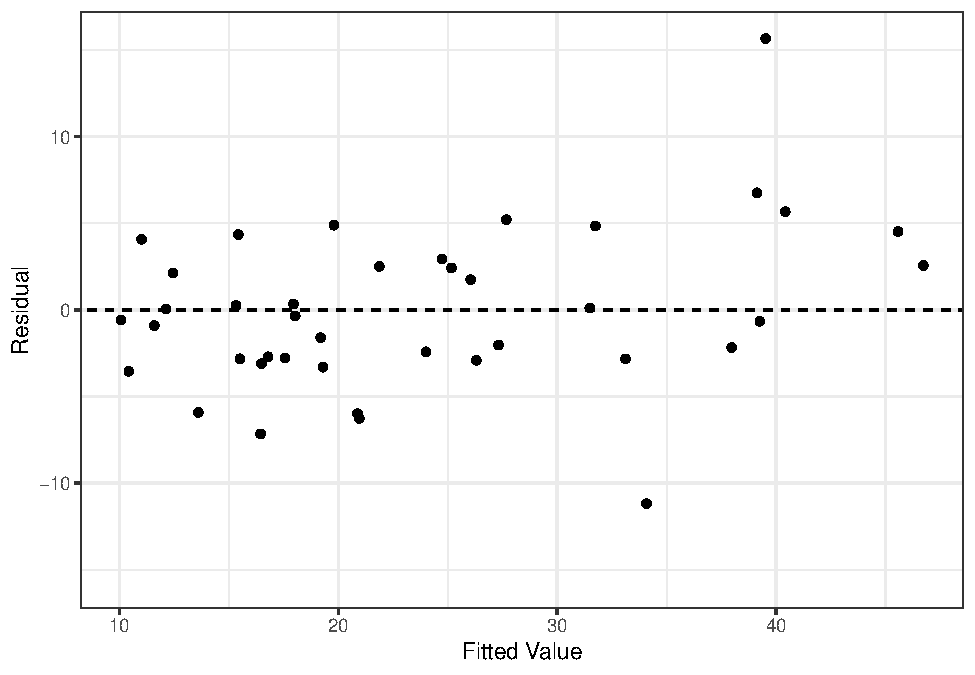
\includegraphics{ch4_files/figure-latex/homoplot-1.pdf}
\caption{Verifying Homoscedasticity}
\end{figure}

\begin{figure}
\centering
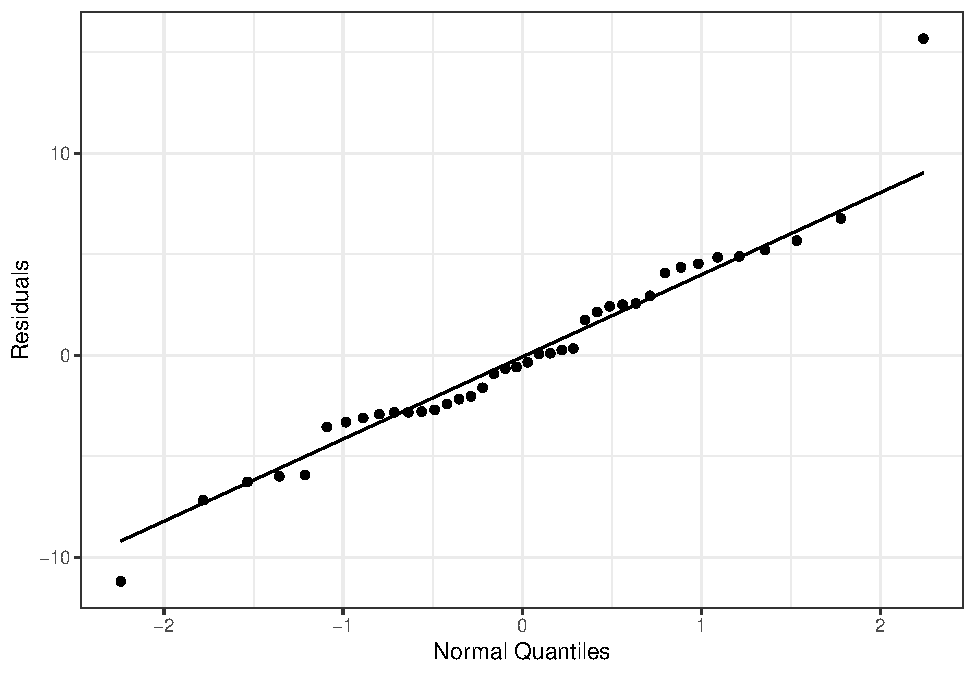
\includegraphics{ch4_files/figure-latex/qqplot-1.pdf}
\caption{Q-Q Plot}
\end{figure}

Excluding a few outliers, figures \ref{fig:homoplot} and
\ref{fig:qqplot} show nothing to suggest that the assumptions of
homoscedasticity and normality were violated.

\subsubsection{Adjusted Means}\label{adjusted-means}

Finally, we can report the adjusted means. The
\texttt{emmeans::emmeans()} function provides adjusted means, taking as
input the model and variable by which to separate the means. The results
are shown in table \ref{tab:emmeans-table}.

\begin{Shaded}
\begin{Highlighting}[]
\FunctionTok{library}\NormalTok{(emmeans)}
\NormalTok{emm }\OtherTok{\textless{}{-}} \FunctionTok{emmeans}\NormalTok{(mixed.model, }\SpecialCharTok{\textasciitilde{}}\NormalTok{ Sequence)}
\end{Highlighting}
\end{Shaded}

\begin{table}

\caption{\label{tab:emmeans-table}LS Means}
\centering
\begin{tabular}[t]{lrrrrr}
\toprule
Sequence & emmean & SE & df & lower.CL & upper.CL\\
\midrule
C-B & 24.55 & 3.87 & 18 & 16.42 & 32.68\\
B-C & 23.12 & 3.87 & 18 & 14.99 & 31.25\\
\bottomrule
\end{tabular}
\end{table}

\section{Using Baseline Measurements}\label{using-baseline-measurements}

\subsection{Data Structure}\label{data-structure-1}

The study also measured insulin levels before ingestion, so we can
incorporate these baseline measurements into the analysis. The format of
the data with baseline (Pre) and post-ingestion insulin levels (Post) is
shown in table \ref{tab:data-demo-baseline}. For summaries and
modelling, we need the data also in `longer' and `wider' formats, shown
in tables \ref{tab:data-wide-demo-baseline} and
\ref{tab:data-long-demo-baseline}.

\begin{table}

\caption{\label{tab:data-demo-baseline}Subsample of Data with Baselines}
\centering
\begin{tabular}[t]{llllrr}
\toprule
Subject & Sequence & Period & Treatment & Pre & Post\\
\midrule
1 & C-B & 1 & CRICKET & 20.3 & 18.3\\
1 & C-B & 2 & BEEF & 14.6 & 14.1\\
2 & C-B & 1 & CRICKET & 11.1 & 14.7\\
2 & C-B & 2 & BEEF & 11.1 & 24.7\\
4 & C-B & 1 & CRICKET & 38.3 & 45.9\\
\bottomrule
\end{tabular}
\end{table}

\begin{Shaded}
\begin{Highlighting}[]
\NormalTok{data.long }\OtherTok{\textless{}{-}}\NormalTok{ data }\SpecialCharTok{\%\textgreater{}\%}
  \FunctionTok{pivot\_longer}\NormalTok{(}\AttributeTok{cols =} \FunctionTok{c}\NormalTok{(Pre,Post),}
               \AttributeTok{names\_to =} \StringTok{"Measurement"}\NormalTok{,}
               \AttributeTok{values\_to =} \StringTok{"Insulin"}\NormalTok{,}
               \AttributeTok{names\_transform =}\NormalTok{ as\_factor)}

\NormalTok{data.wide }\OtherTok{\textless{}{-}}\NormalTok{ data }\SpecialCharTok{\%\textgreater{}\%}
  \FunctionTok{pivot\_wider}\NormalTok{(}\AttributeTok{id\_cols =} \FunctionTok{c}\NormalTok{(Subject, Sequence),}
              \AttributeTok{names\_from =}\NormalTok{ Period, }\AttributeTok{values\_from =} \FunctionTok{c}\NormalTok{(Pre, Post)) }\SpecialCharTok{\%\textgreater{}\%}
  \FunctionTok{relocate}\NormalTok{(Post\_1, }\AttributeTok{.after =} \StringTok{"Pre\_1"}\NormalTok{)}
\end{Highlighting}
\end{Shaded}

\begin{table}

\caption{\label{tab:data-wide-demo-baseline}Subsample of Data with Baselines in 'Wider' Format}
\centering
\begin{tabular}[t]{llrrrr}
\toprule
Subject & Sequence & Pre\_1 & Post\_1 & Pre\_2 & Post\_2\\
\midrule
1 & C-B & 20.3 & 18.3 & 14.6 & 14.1\\
2 & C-B & 11.1 & 14.7 & 11.1 & 24.7\\
4 & C-B & 38.3 & 45.9 & 51.6 & 35.8\\
5 & C-B & 40.3 & 46.1 & 51.8 & 38.6\\
7 & C-B & 24.6 & 17.6 & 31.3 & 17.7\\
\bottomrule
\end{tabular}
\end{table}

\begin{table}

\caption{\label{tab:data-long-demo-baseline}Subsample of Data with Baselines in 'Longer' Format}
\centering
\begin{tabular}[t]{lllllr}
\toprule
Subject & Sequence & Period & Treatment & Measurement & Insulin\\
\midrule
1 & C-B & 1 & CRICKET & Pre & 20.3\\
1 & C-B & 1 & CRICKET & Post & 18.3\\
1 & C-B & 2 & BEEF & Pre & 14.6\\
1 & C-B & 2 & BEEF & Post & 14.1\\
\bottomrule
\end{tabular}
\end{table}

For modelling, we also need to calculate the difference in baselines for
each subject. Using a host of functions from the \texttt{dplyr} package,
we first calculate the difference in the `wider' format, before using
\texttt{pivot\_longer()} to transform the data into the format needed
for implementing the model. The resulting data is shown in table \ref{}

\begin{Shaded}
\begin{Highlighting}[]
\NormalTok{data.baselines }\OtherTok{\textless{}{-}}\NormalTok{ data.wide }\SpecialCharTok{\%\textgreater{}\%}
  \FunctionTok{mutate}\NormalTok{(}\AttributeTok{baseline\_diff =}\NormalTok{ Pre\_1 }\SpecialCharTok{{-}}\NormalTok{ Pre\_2) }\SpecialCharTok{\%\textgreater{}\%}
  \FunctionTok{rename}\NormalTok{(}\StringTok{\textasciigrave{}}\AttributeTok{1}\StringTok{\textasciigrave{}} \OtherTok{=} \StringTok{"Post\_1"}\NormalTok{, }\StringTok{\textasciigrave{}}\AttributeTok{2}\StringTok{\textasciigrave{}} \OtherTok{=} \StringTok{"Post\_2"}\NormalTok{) }\SpecialCharTok{\%\textgreater{}\%}
  \FunctionTok{pivot\_longer}\NormalTok{(}\AttributeTok{cols =} \FunctionTok{c}\NormalTok{(}\StringTok{\textasciigrave{}}\AttributeTok{1}\StringTok{\textasciigrave{}}\NormalTok{,}\StringTok{\textasciigrave{}}\AttributeTok{2}\StringTok{\textasciigrave{}}\NormalTok{), }\AttributeTok{names\_to =} \StringTok{"Period"}\NormalTok{, }\AttributeTok{values\_to =} \StringTok{"Post"}\NormalTok{,}
               \AttributeTok{names\_transform =}\NormalTok{ as\_factor) }\SpecialCharTok{\%\textgreater{}\%}
  \FunctionTok{select}\NormalTok{(Subject, Period, baseline\_diff) }\SpecialCharTok{\%\textgreater{}\%} 
  \FunctionTok{inner\_join}\NormalTok{(data, }\FunctionTok{join\_by}\NormalTok{(Subject }\SpecialCharTok{==}\NormalTok{ Subject, Period }\SpecialCharTok{==}\NormalTok{ Period)) }\SpecialCharTok{\%\textgreater{}\%}
  \FunctionTok{relocate}\NormalTok{(Sequence, }\AttributeTok{.after =} \StringTok{"Subject"}\NormalTok{) }\SpecialCharTok{\%\textgreater{}\%}
  \FunctionTok{relocate}\NormalTok{(baseline\_diff, }\AttributeTok{.after =} \StringTok{"Post"}\NormalTok{)}
\end{Highlighting}
\end{Shaded}

\begin{table}

\caption{\label{tab:data-baseline-demo}Subsample of Data with Baseline Differences}
\centering
\begin{tabular}[t]{llllrrr}
\toprule
Subject & Sequence & Period & Treatment & Pre & Post & baseline\_diff\\
\midrule
1 & C-B & 1 & CRICKET & 20.3 & 18.3 & 5.7\\
1 & C-B & 2 & BEEF & 14.6 & 14.1 & 5.7\\
2 & C-B & 1 & CRICKET & 11.1 & 14.7 & 0.0\\
2 & C-B & 2 & BEEF & 11.1 & 24.7 & 0.0\\
4 & C-B & 1 & CRICKET & 38.3 & 45.9 & -13.3\\
\bottomrule
\end{tabular}
\end{table}

\subsection{Summarising with
Baselines}\label{summarising-with-baselines}

The summary table can be expanded to include the baseline measurements,
as shown in table \ref{tab:table1-baseline}.

\begin{table}
\centering
\caption{\label{tab:table1-baseline}Summary Table with Baseline Values (Pre)}
\centering
\resizebox{\ifdim\width>\linewidth\linewidth\else\width\fi}{!}{
\begin{tabular}[t]{l>{}r|rrr>{}r|rrrrrrrr}
\toprule
\multicolumn{2}{c}{ } & \multicolumn{4}{c}{Overall} & \multicolumn{4}{c}{Period 1} & \multicolumn{4}{c}{Period 2} \\
\cmidrule(l{3pt}r{3pt}){3-6} \cmidrule(l{3pt}r{3pt}){7-10} \cmidrule(l{3pt}r{3pt}){11-14}
\multicolumn{2}{c}{ } & \multicolumn{2}{c}{Pre} & \multicolumn{2}{c}{Post} & \multicolumn{2}{c}{Pre} & \multicolumn{2}{c}{Post} & \multicolumn{2}{c}{Pre} & \multicolumn{2}{c}{Post} \\
\cmidrule(l{3pt}r{3pt}){3-4} \cmidrule(l{3pt}r{3pt}){5-6} \cmidrule(l{3pt}r{3pt}){7-8} \cmidrule(l{3pt}r{3pt}){9-10} \cmidrule(l{3pt}r{3pt}){11-12} \cmidrule(l{3pt}r{3pt}){13-14}
Sequence & Subject & Mean & SD & Mean & SD & Mean & SD & Mean & SD & Mean & SD & Mean & SD\\
\midrule
C-B & 10 & 25.71 & 13.53 & 24.55 & 14.43 & 24.03 & 10.70 & 25.13 & 16.07 & 27.39 & 16.31 & 23.97 & 13.45\\
B-C & 10 & 27.91 & 14.39 & 23.12 & 11.11 & 29.73 & 18.94 & 25.84 & 13.83 & 26.10 & 8.44 & 20.40 & 7.27\\
\midrule\\
Total & 20 & 26.81 & 13.83 & 23.84 & 12.74 & 26.88 & 15.25 & 25.48 & 14.60 & 26.75 & 12.66 & 22.18 & 10.68\\
\bottomrule
\end{tabular}}
\end{table}

We can also extend the boxplot to incorporate the baseline measurements
(see figure \ref{fig:boxplot-with-baseline}.

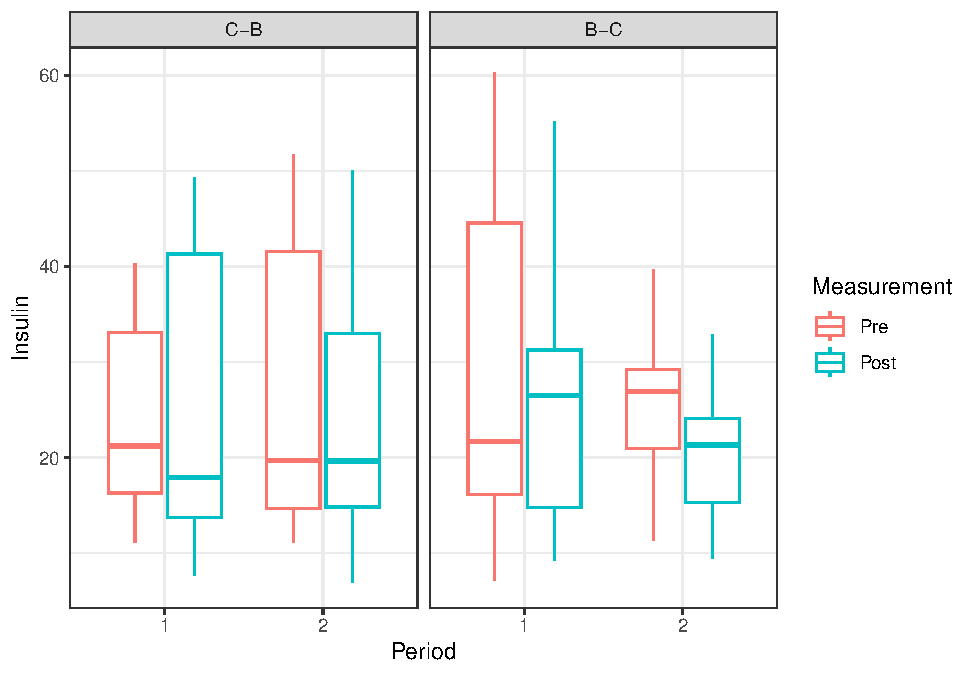
\includegraphics{ch4_files/figure-latex/boxplot-with-baseline-1.pdf}

\subsection{Modelling with Baselines}\label{modelling-with-baselines}

First we construct the ANOVA table, this time including the baseline by
period interaction, as shown in table \ref{tab:anova-table-baseline}.

\begin{Shaded}
\begin{Highlighting}[]
\NormalTok{anova.table.baseline }\OtherTok{\textless{}{-}} \FunctionTok{aov}\NormalTok{(Post }\SpecialCharTok{\textasciitilde{}}\NormalTok{ Treatment }\SpecialCharTok{+}\NormalTok{ Period }\SpecialCharTok{*}\NormalTok{ baseline\_diff }\SpecialCharTok{+}\NormalTok{ Sequence }\SpecialCharTok{+}\NormalTok{ Subject,}
                             \AttributeTok{data =}\NormalTok{ data.baselines) }\SpecialCharTok{\%\textgreater{}\%}
  \FunctionTok{summary}\NormalTok{()}
\end{Highlighting}
\end{Shaded}

We update the mixed model to include the period-by-baseline difference
interaction. Estimates are shown in table
\ref{tab:mixed-model-baseline}, and the updated LS means in table
\ref{tab:emmeans-baseline}.

\begin{Shaded}
\begin{Highlighting}[]
\NormalTok{mixed.model.baselines }\OtherTok{\textless{}{-}} \FunctionTok{lmer}\NormalTok{(Post }\SpecialCharTok{\textasciitilde{}}\NormalTok{ Treatment }\SpecialCharTok{+}\NormalTok{ Period }\SpecialCharTok{*}\NormalTok{ baseline\_diff }\SpecialCharTok{+}\NormalTok{ Sequence }\SpecialCharTok{+}\NormalTok{ (}\DecValTok{1}\SpecialCharTok{|}\NormalTok{Subject),}
              \AttributeTok{data =}\NormalTok{ data.baselines)}
\end{Highlighting}
\end{Shaded}

\begin{table}

\caption{\label{tab:emmeans-baseline}LS Means}
\centering
\begin{tabular}[t]{lrrrrr}
\toprule
Sequence & emmean & SE & df & lower.CL & upper.CL\\
\midrule
C-B & 24.01 & 4.03 & 17 & 15.49 & 32.52\\
B-C & 23.66 & 4.03 & 17 & 15.15 & 32.18\\
\bottomrule
\end{tabular}
\end{table}
